Official statistics published by the U.S. government~\cite{EducationPaysBureau} indicate that individuals with doctoral degrees belong to a distinguished group characterized by the highest median weekly earnings and the lowest unemployment rates across the country. With the privilege comes responsibility. In recognizing the advantages my educational status affords me, I am committed to leveraging this privilege to foster the excellence of each individual that I mentor from a diverse student body at the \appSchool{}.

I acutely recognize that \emph{diversity} in academia extends beyond common identity indicators and also includes educational backgrounds and life experiences. Drawing from my personal history as an international graduate student and a parent during postdoctoral training, I share a commonality with many students alike regarding their academic and life challenges, and I keenly would like to listen to the needs of students from an even broader spectrum of backgrounds, such as those of transfer students, non-traditional students (e.g., aged 25 and above or those returning to education), student parents, first-generation students, academically under-prepared students, and so on. Capturing this full spectrum is essential to crafting a truly inclusive educational environment.


This commitment became even more tangible during a routine COVID test on campus. The young man conducting the test was unaware of what a ``postdoc'' was, revealing a gap in his knowledge of educational pathways, especially regarding doctoral programs and beyond. This interaction keeps on reminding me of the broader role that an educator can play. As a future faculty member, I am inspired to be a force of enlightenment and change, to open up opportunities to students who may have never known of the intellectual and life options that abound at our university. The influence of these seemingly simple acts of sharing knowledge and opening doors can be more significant than most people perceive.

\begin{figure}[!ht]
    \centering
    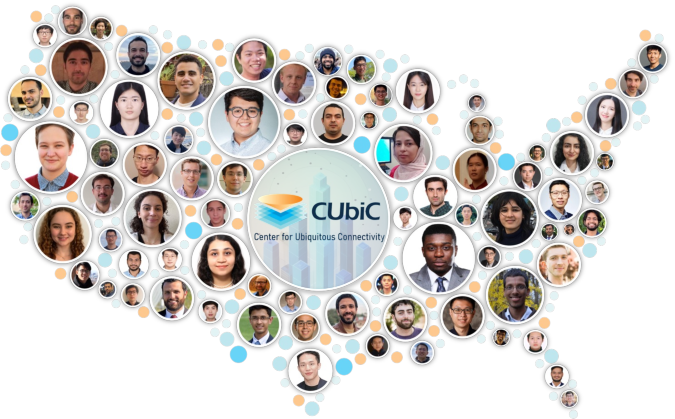
\includegraphics[width=0.4\linewidth]{../../fig/diversity.pdf}
    \caption{Firsthand experience of diversity in action at the SRC JUMP 2.0 Center for Ubiquitous Connectivity (CUbiC) have profoundly shaped my understanding of inclusive mentoring practices.}
    \label{fig:diversity}
\end{figure}

My time at the Center for Ubiquitous Connectivity (CUbiC) under the SRC JUMP 2.0 program has been instrumental in shaping my understanding of practical diversity in action. Diversity is a critical priority in the CUbiC center, as evidenced by the center featuring a female director, a female theme lead, 6 female principal investigators, alongside over 20\% and growing researchers from underrepresented groups. Witnessing the center's inclusive mentoring and outreach programs has demonstrated to me the utmost importance of such initiatives in a research environment. These experiences have provided me with a solid framework for what I aspire to emulate in establishing my own research group in the \appDept{} at the \appSchool{}. In light of these experiences, I formulate my mentoring philosophy guided by a series of introspective questions:

\paragraph{How would I mentor students from different background and with different research interests/career aspirations?}
My approach will be student-adapted. An essential part of my mentoring role beyond giving guidance is to listen to and understand the students' needs, and to create a supportive and collaborative research environment where they can focus and not be distracted by other concerns. At the beginning, I expect to work as closely as possible with them, to learn about their interests and needs, as well as providing more detailed guidance. As they acquire a more holistic understanding of the field and formulate their own research directions, I will encourage them to explore their own ideas and collaborate with other fellow students and researchers, while being available for consultation and feedback. I will also adjust my mentoring approach over the course of a student's progress as they formulate their career aspirations and expose them with the necessary training opportunities, such as internships and/or teaching,  to acquire the necessary skills to achieve their goals.

\paragraph{How would I plan to meet with students on their progress?}
I understand that students have different styles of practice in learning and research, but we also need to work together toward common goals such as project deliverables, publications, and pushing the technology forward. In light of this, I plan to have a hybrid of group meetings, project-specific meetings, and one-on-one meetings with students. The weekly group meetings are for individuals to share the progress with the group and to gather feedback from other brilliant minds. The weekly project-specific meetings, usually in the form of a smaller group, will dive deeper into the technical details of the projects and ensure progress. The one-on-one meetings are where things get more diverse in frequency and topics. While I generally suggest bi-weekly, I also encourage students to judge on their own pace and reach out anytime if they need. Topics on one-on-one meetings could range from research progress and technical questions, to career advice and other concerns should they wish to bring up, and I will provide my perspective from my own experience and/or point them to the right resources if needed.

\paragraph{How would I stay available for students' requests?}
I would expect the formal requests and important updates to be communicated via email, which I usually respond within hours or provide a timeframe for a more detailed follow-up. However, I am also proficient with other communication channels such as Slack, and recognizing the trend in younger generations to prefer more instant communication platforms, such as Discord. In light of the post-Covid era where a hybrid of in-person and remote collaboration has become the new norm, I am committed to expand and adapt my reachability to maximize the efficiency of communication.

\paragraph{What are my general expectations for students' graduation?}




In conclusion, it is through the combined efforts\textemdash recognizing the full spectrum of diversity, actively contributing to an inclusive academic culture, and taking every opportunity to educate and inform\textemdash that I aim to fulfill the responsibility that accompanies my privileged educational achievement. I see it as my duty to ensure that the pathways to academic and professional success are accessible to all, and to serve as a mentor for the next generation of scholars and innovators.

